% Étape 4 : calibration. Sources : notebooks/04_calibration.ipynb, results/calibration_*.csv, results/figures/etape4_calibration_spx.png, data/spx_surface.npz.

\section{Calibration et seuil de rentabilité}
\label{sec-calibration}

Dans cette dernière étape, nous utilisons le réseau retenu ($2 \times 128$ neurones, initialisation de He,
activation GELU, entraîné avec Adam) pour de vraies calibrations, et nous le comparons au pricer de référence par
transformée de Fourier (méthode COS).

\subsection{Protocole expérimental}

Le réseau et Fourier utilisent le même optimiseur, pour que seule la façon de calculer une surface change :
Levenberg-Marquardt, avec la fonction \texttt{least\_squares} de SciPy. Les bornes des cinq paramètres
$\Theta = (v_0, \theta, \kappa, \xi, \rho)$ sont imposées par un changement de variable sigmoïde, et les points
manquants (\texttt{NaN}) de la surface cible sont ignorés dans les résidus. Chaque calibration part des mêmes
$N_{\text{starts}} = 5$ points de départ, tirés par hypercube latin (graine $0$).

\subsection{Calibration sur surfaces simulées}

Nous comparons d'abord les deux méthodes sur $100$ surfaces du jeu de test (graine $42$), dont nous connaissons les
vrais paramètres $\Theta^*$. Le \cref{tab-calib-simulee} donne le taux de convergence, l'erreur d'ajustement sur les
volatilités implicites (en points de base, $1~\text{pb} = 10^{-4}$), l'erreur relative sur chaque paramètre
(rapportée à la largeur de sa plage) et le temps de calcul complet.

\begin{table}[htbp]
\centering
\caption{Performances comparées de la calibration sur $100$ surfaces du jeu de test ($5$ points de départ par surface).}
\label{tab-calib-simulee}
\small
\setlength{\tabcolsep}{4pt}
\begin{tabular}{lcccccc}
\toprule
 & \multicolumn{3}{c}{\textbf{Réseau de neurones}} & \multicolumn{3}{c}{\textbf{Fourier (COS Python)}} \\
\cmidrule(lr){2-4} \cmidrule(lr){5-7}
\textbf{Métrique} & \textbf{Moyenne} & \textbf{Médiane} & \textbf{Max} & \textbf{Moyenne} & \textbf{Médiane} & \textbf{Max} \\
\midrule
Taux de convergence & \multicolumn{3}{c}{$100\,\%$} & \multicolumn{3}{c}{$100\,\%$} \\
Erreur d'ajustement (pb) & $1{,}25$ & $1{,}12$ & $3{,}09$ & $2{,}23$ & $0{,}00$ & $67{,}60$ \\
Erreur maximale (pb) & $5{,}18$ & $4{,}59$ & $14{,}89$ & $10{,}28$ & $0{,}00$ & $212{,}80$ \\
Temps par calibration (s) & $0{,}0541$ & $0{,}0445$ & $0{,}3820$ & $34{,}8128$ & $25{,}3025$ & $173{,}5981$ \\
Nombre d'évaluations & $359{,}0$ & $330{,}0$ & $3097{,}0$ & $793{,}1$ & $611{,}5$ & $2654{,}0$ \\
\midrule
Erreur relative $v_0$ (\%) & $0{,}11\,\%$ & $0{,}08\,\%$ & $0{,}63\,\%$ & $0{,}25\,\%$ & $0{,}00\,\%$ & $4{,}19\,\%$ \\
Erreur relative $\theta$ (\%) & $0{,}08\,\%$ & $0{,}05\,\%$ & $1{,}35\,\%$ & $0{,}10\,\%$ & $0{,}00\,\%$ & $4{,}70\,\%$ \\
Erreur relative $\kappa$ (\%) & $0{,}33\,\%$ & $0{,}22\,\%$ & $1{,}90\,\%$ & $1{,}53\,\%$ & $0{,}00\,\%$ & $36{,}17\,\%$ \\
Erreur relative $\xi$ (\%) & $0{,}17\,\%$ & $0{,}15\,\%$ & $0{,}75\,\%$ & $0{,}56\,\%$ & $0{,}00\,\%$ & $9{,}86\,\%$ \\
Erreur relative $\rho$ (\%) & $0{,}36\,\%$ & $0{,}17\,\%$ & $4{,}67\,\%$ & $1{,}06\,\%$ & $0{,}00\,\%$ & $17{,}12\,\%$ \\
\bottomrule
\end{tabular}
\end{table}

Une calibration complète prend en moyenne $54{,}1~\text{ms}$ avec le réseau, contre $34{,}81~\text{s}$ avec le
pricer Fourier en Python : le réseau va $643{,}6$ fois plus vite. Le gain a deux origines. Le réseau évalue une
surface en NumPy pur en $0{,}176~\text{ms}$, normalisation par les scalers et mise en forme des tableaux comprises ;
la passe avant elle-même n'en prend que $0{,}028~\text{ms}$. Sa surface est aussi plus lisse, et l'optimiseur a
besoin de deux fois moins d'évaluations ($359$ contre $793$).

La précision ne se dégrade pas pour autant. L'erreur d'ajustement du réseau est de $1{,}12~\text{pb}$ en médiane
($1{,}25~\text{pb}$ en moyenne), bien en deçà des écarts observables sur les marchés d'options, et les cinq
paramètres sont retrouvés à moins de $0{,}22\,\%$ de la largeur de leur domaine en médiane.

Fourier atteint $0{,}00~\text{pb}$ en médiane, ce qui est attendu : les surfaces de test ont été générées par ce même
modèle. Il reste en revanche sensible à des minima locaux sur certaines configurations extrêmes, où son erreur
monte jusqu'à $67{,}60~\text{pb}$. Celle du réseau ne dépasse pas $3{,}09~\text{pb}$ sur tout le jeu de test.

\subsection{Calibration sur données de marché (SPX)}

Nous calibrons ensuite avec les deux méthodes les quatre surfaces réelles d'options sur l'indice S\&P 500 de
\texttt{spx\_surface.npz} ($3$, $4$, $5$ et $20$ novembre), restreintes à la zone de calibration de la
\cref{sec-spx} : $K/F \in [0{,}7\,;\,1{,}3]$ et $T \ge 0{,}3~\text{an}$, soit $46$ à $49$ points valides sur $88$
selon la date. Cette zone écarte les maturités très courtes, où le modèle de Heston ne parvient pas à reproduire le
\textit{skew} prononcé du marché.

\begin{table}[htbp]
\centering
\caption{Calibration comparée sur les quatre surfaces réelles SPX ($5$ points de départ par surface).}
\label{tab-calib-spx}
\resizebox{\textwidth}{!}{%
\begin{tabular}{llccccccccc}
\toprule
\textbf{Date} & \textbf{Méthode} & \textbf{Err. moy. (pb)} & \textbf{Err. max (pb)} & \textbf{Temps (s)} & \textbf{Éval.} & $v_0$ & $\theta$ & $\kappa$ & $\xi$ & $\rho$ \\
\midrule
2026-11-03 & Réseau & $28{,}57$ & $145{,}59$ & $0{,}173$ & $635$ & $0{,}0361$ & $0{,}0495$ & $3{,}8965$ & $1{,}5000$ & $-0{,}7187$ \\
 & Fourier & $29{,}20$ & $146{,}14$ & $33{,}831$ & $397$ & $0{,}0362$ & $0{,}0493$ & $3{,}8851$ & $1{,}5000$ & $-0{,}7195$ \\
\midrule
2026-11-04 & Réseau & $28{,}58$ & $124{,}18$ & $0{,}043$ & $358$ & $0{,}0230$ & $0{,}0486$ & $3{,}9827$ & $1{,}5000$ & $-0{,}7122$ \\
 & Fourier & $29{,}49$ & $125{,}18$ & $39{,}762$ & $438$ & $0{,}0231$ & $0{,}0485$ & $3{,}9944$ & $1{,}5000$ & $-0{,}7131$ \\
\midrule
2026-11-05 & Réseau & $28{,}51$ & $165{,}27$ & $0{,}132$ & $1094$ & $0{,}0526$ & $0{,}0507$ & $3{,}8410$ & $1{,}5000$ & $-0{,}7509$ \\
 & Fourier & $29{,}05$ & $165{,}70$ & $27{,}160$ & $427$ & $0{,}0530$ & $0{,}0505$ & $3{,}8145$ & $1{,}5000$ & $-0{,}7518$ \\
\midrule
2026-11-20 & Réseau & $29{,}22$ & $123{,}17$ & $0{,}034$ & $272$ & $0{,}0760$ & $0{,}0555$ & $3{,}9106$ & $1{,}5000$ & $-0{,}7597$ \\
 & Fourier & $29{,}85$ & $123{,}72$ & $35{,}644$ & $466$ & $0{,}0764$ & $0{,}0552$ & $3{,}8858$ & $1{,}5000$ & $-0{,}7614$ \\
\bottomrule
\end{tabular}%
}
\end{table}

Sur les quatre jours, le réseau donne les mêmes calibrations que Fourier (\cref{tab-calib-spx},
\cref{fig-calib-spx}). Les paramètres sont presque identiques d'une méthode à l'autre : l'écart est inférieur à
$0{,}0005$ sur $v_0$ et $\theta$, et à $0{,}0018$ sur $\rho$. L'erreur d'ajustement au marché est la même, entre
$28{,}5$ et $29{,}8~\text{pb}$ environ ; elle vient des limites du modèle de Heston à deux facteurs, pas du réseau.
Le temps moyen par journée passe en revanche de $34{,}10~\text{s}$ à $0{,}095~\text{s}$ : le réseau va environ
$360$ fois plus vite, et plus de $1000$ fois le 20 novembre.

\begin{figure}[htbp]
\centering
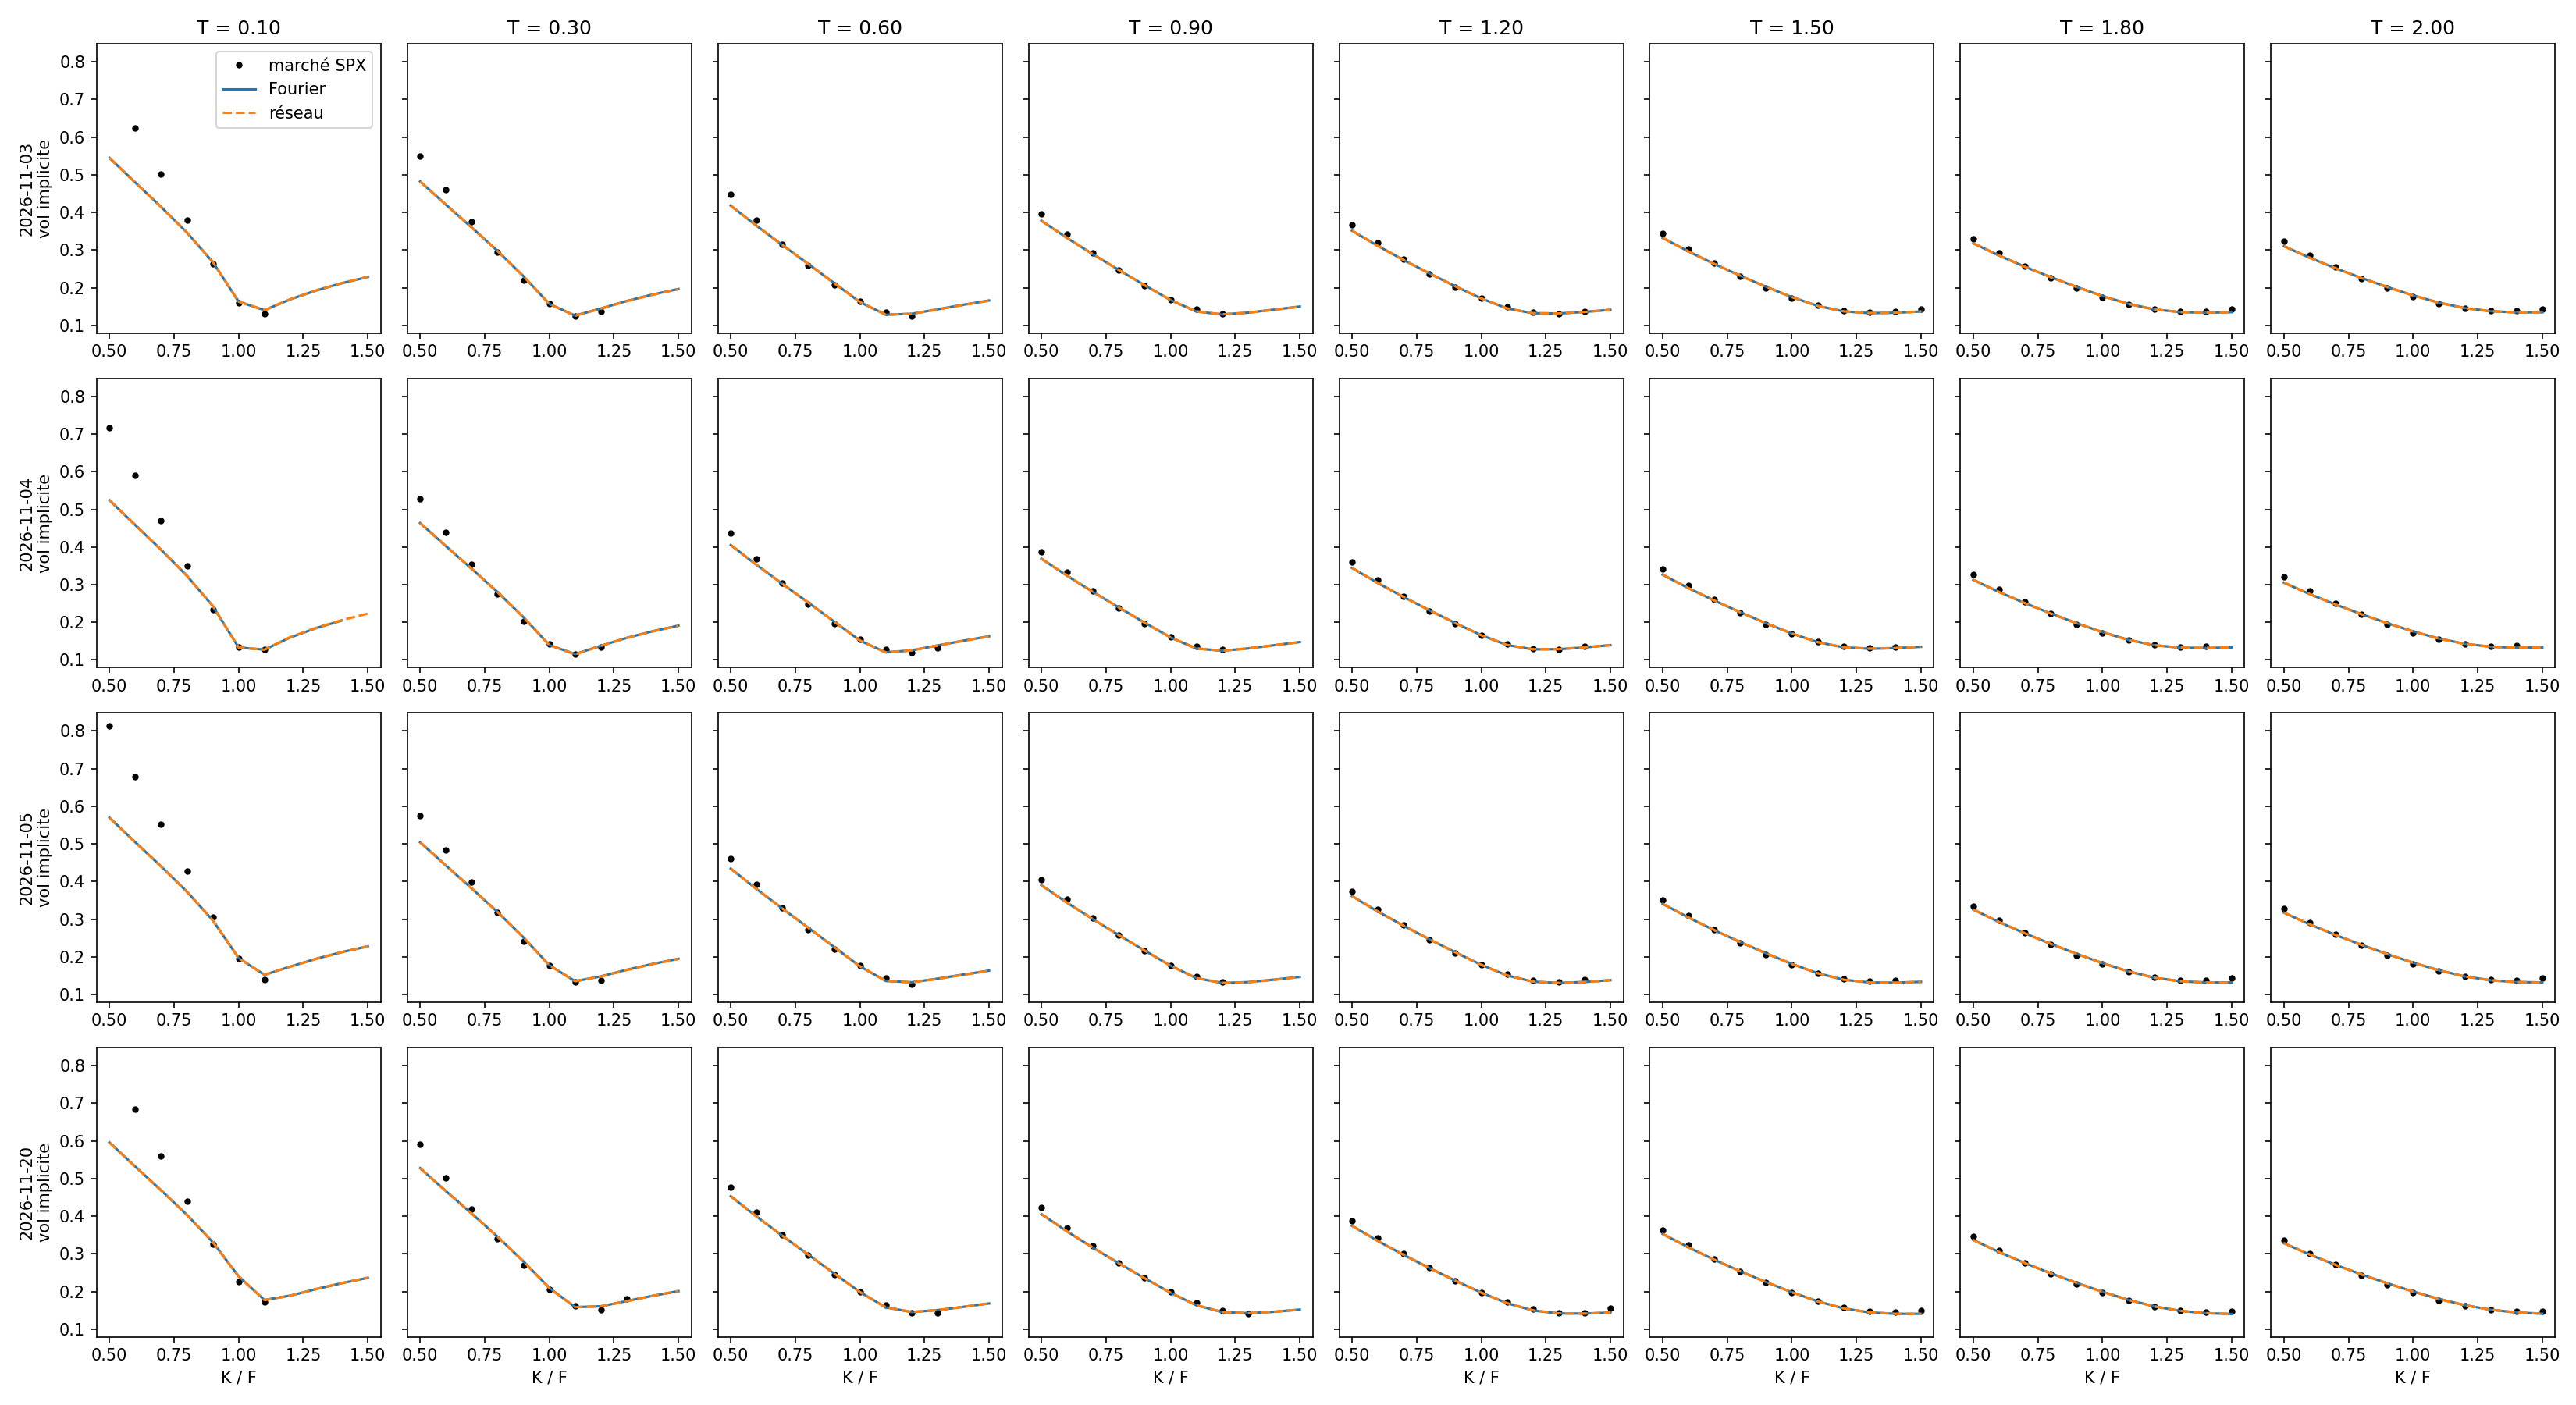
\includegraphics[width=\textwidth]{../results/figures/etape4_calibration_spx.png}
\caption{Superposition des volatilités implicites du marché SPX et des surfaces calibrées par Fourier et par le réseau de neurones sur les quatre dates étudiées.}
\label{fig-calib-spx}
\end{figure}

\subsection{Seuil de rentabilité}

Le réseau a un coût fixe, payé une seule fois : la génération des $50\,000$ surfaces d'apprentissage
($T_{\text{génération}} = 23{,}9~\text{s}$ en Julia) et l'entraînement du modèle final
($T_{\text{entraînement}} = 136{,}0~\text{s}$), soit $159{,}9~\text{s}$ au total. Le seuil de rentabilité $n^*$ est
le nombre de calibrations à partir duquel ce coût est amorti :
\begin{equation}
n^* = \left\lceil \frac{T_{\text{génération}} + T_{\text{entraînement}}}{t_{\text{calib, Fourier}} - t_{\text{calib, réseau}}} \right\rceil
\end{equation}

Avec les temps moyens mesurés sur le jeu de test ($t_{\text{calib, Fourier}} = 34{,}813~\text{s}$ et
$t_{\text{calib, réseau}} = 0{,}0541~\text{s}$), chaque calibration fait gagner $34{,}76~\text{s}$, et le seuil vaut :
\[
n^* = \left\lceil \frac{23{,}9 + 136{,}0}{34{,}813 - 0{,}0541} \right\rceil = 5 \text{ calibrations} \quad (\text{valeur exacte } 4{,}60).
\]
Si l'on compare plutôt au pricer de référence en Julia ($2{,}29~\text{ms}$ par surface sur un cœur, soit environ
$1{,}82~\text{s}$ pour $793$ évaluations), le gain tombe à $1{,}76~\text{s}$ par calibration, et le réseau est
rentable à partir de $n^* = 91$ calibrations. En production, ce volume est atteint dès la première journée de
cotation.
